\section{Networking}\label{networking}
For the last, individual milestone, I implemented a network stack for our operating system, consisting of an ethernet driver, a library for networking functionalities, and a small selection of simple applications employing this library. While still missing some of the functionality found in modern commercial operating systems, my network stack does already provide a list of useful features. It handles many of the low-level processes and protocols necessary for successful communication with other devices, and it provides a more high-level interface for applications to make use of the Toradex board's integrated Ethernet adapter.

\subsection{Overview}
The Ethernet driver functions as a process running in userspace. It is invoked from our init process and is given special permissions to access the Toradex board's networking hardware. The driver interacts with the networking hardware through two special queues, called device-queues. One of these queues is used to enqueue packets that are to be sent from the device, while the driver can dequeue packets from the other queue once they have been received by the device.

See Listing \ref{enet:driverstate} for a short overview of the ethernet driver's state, including some of the attributes it uses to provide all its features.

\begin{code}
\begin{mdframed}[style=myframe]
\begin{minted}[xleftmargin=\parindent,linenos,breaklines]{C}
// struct to represent a single udp packet in a receive-buffer
struct udp_recv_elem {
    void *data;
    // ...
    struct udp_recv_elem *next;
};

struct aos_udp_socket {
    //...
    uint16_t l_port;  // local port
    struct udp_recv_elem *receive_buffer;
    // ...
    struct aos_udp_socket* next;
};

struct aos_icmp_socket {
    uint32_t ip;
    // ...
    struct aos_icmp_socket *next;
};

struct enet_driver_state {
    // ...
    collections_hash_table* arp_table;  // arp-table: mac -> ip
    collections_hash_table* inv_table;  // inverse arp-table: ip -> mac
    struct enet_qstate* send_qstate;  // regionmanager for send-queue

    struct aos_udp_socket *sockets;  // active udp sockets
    struct aos_icmp_socket *pings;  // acive icmp sockets
};
\end{minted}
\end{mdframed}
\caption{State of the Ethernet Driver.}
\end{code}
\label{enet:driverstate}

\subsection{Region Manager}
The device queues used to interact with our networking hardware accept packets in the representation of \C{struct devq\_buff} instances. Each such packet is identified by the region it is stored in, its offset into that region, and its total length. But since the queues themselves do not track which packets are currently enqueued and which are not, the driver needs to employ the region-manager library (\emph{see listing \ref{enet:qstate}}).

The ethernet driver's state has a pointer of type \C{struct enet\_qstate*} under which it tracks which buffers are currently enqueued in its send-queue, and which are not. The region-manager library furthermore provides methods to obtain references to free \C{devq\_buff} instances, and to enqueue a buffer to be sent over the device's network connection. All of this is implemented through a simple linked list. The \C{enet\_qstate} struct stores a linked list of all free buffers, as well as a reference to the queue it is associated with. If a free buffer is requested, the region manager library simply returns the head of its linked list. If no free buffers are available at the moment, the region manager first dequeues as many buffers from the send queue as possible, then inserts them into its linked list and finally returns one of them. During this process, the ethernet driver becomes unavailable, preventing any packets from being sent or received, but this only happens every 512th time a buffer is requested. Since the additional waiting time in such an event is almost undetectable from the outside, I did not see the need to be more proactive in dequeueing buffers. Should this become a bigger problem however, the ethernet driver could also be modified to allocate new regions and add them to its send queue if it ever runs out of send buffers.

\begin{code}
\begin{mdframed}[style=myframe]
\begin{minted}[xleftmargin=\parindent,linenos,breaklines]{C}
struct dev_list {
    struct devq_buf* cur;
    struct dev_list* next;
};

// struct to keep track of an entire enet-region
struct enet_qstate {
    struct enet_queue* queue;
    struct dev_list* free;
};

// ...
errval_t get_free_buf(struct enet_qstate* qs, struct devq_buf* ret);

errval_t enqueue_buf(struct enet_qstate* qs, struct devq_buf* buf);
\end{minted}
\end{mdframed}
\caption{The Core Components of the Region Manager Library.}
\end{code}
\label{enet:qstate}

\subsection{ARP}
In order to successfully communicate with other devices, the driver first needs a working implementation of the ARP protocol, capable of both sending and responding to ARP requests. Both of these processes are entirely handled by the driver, meaning any user of our system will never have to manually create ARP messages.

\subsubsection{Sending ARP Responses}
Whenever the Toradex board receives an ARP request addressed to its IP address, the ethernet driver automatically calls a designated handler function. In it, the driver saves the source IP and MAC to its ARP table, fills its own MAC and IP into an ARP response and finally sends its response back over the network.

\subsubsection{Sending ARP Requests}
When the driver attempts to send a packet to any target IP address, it first performs a lookup in its ARP table in order to obtain the corresponding target MAC address. If it cannot find such a MAC address in its own ARP table, it automatically creates an ARP request for that MAC address before returning the error code \C{ENET\_ERR\_ARP\_UNKNOWN}. The driver does however only perform ARP requests when trying to reach an address it cannot find in its ARP table. Therefore, it does not expose a dedicated function just for ARP requests.

\hindsight{
For my ethernet driver, I made very little use of the various struct members for \C{devq\_buffers}. Sinc I only implemented a relatively small number of protocols, never layered deeper than 3 levels, I was still able to achieve all required functionality with regular addresses. Nevertheless, making full use of the additional offsets for \C{devq_buffer} instances, I could have reduced my code duplication by a bit, and also made my driver easier to extend.}

\subsection{ICMP Replies}
Similar to ARP requests, the driver also takes care of all aspects in handling ICMP echo requests. Whenever it receives one, it immediately sends back an according echo response. Notably, this process completely bypasses the driver's state. Both the IP and MAC address for the reply's destination are taken from the received request, without ever consulting or modifying the driver's ARP table. Furthermore, any such exchange takes place without ever being recorded. While network security and forensics were not a concern for this project, these are points that should be addressed before a system like ours becomes employed in a practical scenario.

With correct handling of both ARP and ICMP echo requests, a device connected to the Toradex board is now able to successfully ping it. To do so, the connected device first sends an ARP request to obtain the board's MAC address. After receiving it, the connected device then has all required information to send valid ICMP echo request packets. Listing \ref{enet:pinger} shows a remote machine pinging the Toradex board twice. Before calling \C{ping}, the board's MAC address is not stored on the ARP table, but since \C{ping} causes an ARP exchange, the board's MAC is known afterwards.

\begin{code}
\begin{mdframed}[style=shell]
\bash{sudo arp}\\
Address\ \ \ \ HWtype\ \ HWaddress\ \ \ \ \ \ \ \ \ \ Flags Mask\ \ Iface\\
fritz.box\ \ ether\ \ \ 29:35:a6:2f:10:21\ \ C\ \ \ \ \ \ \ \ \ \ \ wlp2s0\\
\#...\\
\bash{ping 10.0.2.1 -c 2}\\
PING 10.0.2.1 (10.0.2.1) 56(84) bytes of data.\\
64 bytes from 10.0.2.1: icmp\_seq=1 ttl=64 time=0.899 ms\\
64 bytes from 10.0.2.1: icmp\_seq=2 ttl=64 time=0.718 ms\\
\\
--- 10.0.2.1 ping statistics ---\\
2 packets transmitted, 2 received, 0\% packet loss, time 1002ms\\
rtt min/avg/max/mdev = 0.718/0.808/0.899/0.090 ms\\
\bash{sudo arp}\\
Address\ \ \ \ HWtype\ \ HWaddress\ \ \ \ \ \ \ \ \ \ Flags Mask\ \ Iface\\
10.0.2.1\ \ \ ether\ \ \ 00:14:2d:64:13:91\ \ C\ \ \ \ \ \ \ \ \ \ \ enp0s31f6\\
fritz.box\ \ ether\ \ \ 29:35:a6:2f:10:21\ \ C\ \ \ \ \ \ \ \ \ \ \ wlp2s0\\
\#...
\end{mdframed}
\caption{A Remote Machine Pings the Toradex Board}
\end{code}
\label{enet:pinger}

\subsection{UDP Service}
So far, all of the described processes and functionalities have taken place entirely inside the driver. But other programs should of course also be able to access and communicate over the network. For this purpose, the driver exposes the library \C{aos/udp\_service} (\emph{see Listing \ref{enet:udp_service}}). It provides the following core features:

\begin{itemize}
    \item Receiving data arriving in UDP packets on a specified port.
    \item Sending data over UDP through a specified local UDP port and to a specified target IP and port.
    \item Reading the ethernet driver's current ARP table.
    \item Sending ICMP echo requests, resending ones that have not yet been acknowledged.
    \item Receiving ICMP echo replies.
\end{itemize}

\begin{code}
\begin{mdframed}[style=myframe]
\begin{minted}[xleftmargin=\parindent,linenos,breaklines]{C}
errval_t aos_socket_initialize(struct aos_socket *sockref, uint32_t ip_dest, uint16_t f_port, uint16_t l_port);
errval_t aos_socket_send(struct aos_socket *sockref, void *data, uint16_t len);
errval_t aos_socket_send_to(struct aos_socket *sockref, void *data, uint16_t len, uint32_t ip, uint16_t port);
errval_t aos_socket_receive(struct aos_socket *sockref, struct udp_msg *retptr);
errval_t aos_socket_teardown(struct aos_socket *sockref);

errval_t aos_ping_init(struct aos_ping_socket *s, uint32_t ip);
errval_t aos_ping_send(struct aos_ping_socket *s);
uint16_t aos_ping_recv(struct aos_ping_socket *s);

void aos_arp_table_get(char *rtptr);
\end{minted}
\end{mdframed}
\caption{The udp\_service Library}
\end{code}
\label{enet:udp_service}


During startup, the ethernet driver registers itself with the nameserver and any call to the \C{udp\_service} library simply connects to and communicates with the ethernet driver. In order to send or receive any data over UDP, a program must first initialize an \C{aos\_socket} with a target port, a target IP adress, and a local port. If the socket is only used to receive data, or if it should send to various different targets, the target port and target IP address can be left blank:
\begin{mdframed}[style=myframe]
\begin{minted}[xleftmargin=\parindent,linenos,breaklines]{C}
aos_socket sock;
aos_socket_initialize(&sock, 0, 0, 2521);
\end{minted}
\end{mdframed}

This call will instruct the ethernet driver to add a new UDP socket to its driver state (\emph{see listing \ref{enet:driverstate}}). If there already exists a socket with the provided local port, the driver will respond with an error. Otherwise, it will report a success. Whenever the driver receives a UDP packet on a given port, it checks if it has an active UDP socket with that local port. If it does, it stores the received data in the according receive buffer. But if there is no socket listening on that port, the received data will be dropped. It is also worth mentioning that the local port serves as identifier for UDP sockets. A program could therefore hijack a socket created by another program. Possible ways to prevent this include randomized tokens and, of course, capabilities.

After socket initialization, two methods are used to send UDP packets over the network: \C{aos\_socket\_send} and \C{aos\_socket\_send\_to}. They first transmit the payload and destination information to the ethernet driver. When receiving an according request, the driver then verifies the existence of a socket with the specified local port, and it performs a lookup on its ARP table. If it cannot find an according MAC address, it sends an ARP request over the network and reports an error to the calling program. But if it does find a MAC address in its ARP table, it creates a UDP packet with the provided payload to the provided destination. After sending the packet, it reports its success to the caller:
\begin{mdframed}[style=myframe]
\begin{minted}[xleftmargin=\parindent,linenos,breaklines]{C}
errval_t = aos_socket_send_to(&sock, "test", 5, targetip, targetport);
if (!err_is_fail(err)) {
    printf("success!\n");
}
\end{minted}
\end{mdframed}

Figure \ref{fig:enet_send} shows how an application employs this library to send data over UDP to a remote destination. The application successfully initializes a socket and then tries to send a UDP packet over it. Unfortunately, the driver does not have the target IP address in its ARP table. As a result, the driver sends an ARP request to obtain the missing MAC address, and reports this to the calling application. A while later, the application retries to send its data. But since in the meantime the driver has received an ARP response to its previous request, it is now able to successfully send the provided data to its destination.

\begin{figure}[H]
    \centering
    \resizebox{\textwidth}{!} {
        \includesvg{networking/img/Sequence_Send.svg}
        %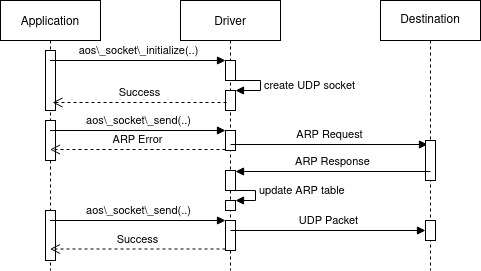
\includegraphics{networking/img/Sequence_Send.png}
    }
    \caption{Creating a Socket and Sending Data to a Remote Destination}
    \label{fig:enet_send}
    
\end{figure}

Receiving data over UDP is quite similar. After initiating a socket for a local port, an application can try to receive data over it. The driver will then check if there are any packets in that port's receive buffer. If there are, the driver will return the oldest one, and if the receive buffer is empty, the driver will report an according error:
\begin{mdframed}[style=myframe]
\begin{minted}[xleftmargin=\parindent,linenos,breaklines]{C}
struct *udp_msg = malloc(sizeof(struct udp_msg) + 2048);
errval_t err = aos_socket_receive(&sock, msg);
if (!err_is_fail(err)) {
    printf("received: \%s\n", msg->data);
}
\end{minted}
\end{mdframed}

Figure \ref{fig:enet_recv} shows an application trying to receive data over an already established socket. The first attempt fails as there is no data in its receive buffer. But afterwards, the driver receives data from a remote source which it then adds to the socket's receive buffer. Finally, the application's second attempt at receiving data succeeds, as now there is a packet in its receive buffer.

\begin{figure}[H]
\centering
    %\scalebox{0.9} {
    \resizebox{\textwidth}{!} {
        \includesvg{networking/img/Sequence_Receive.svg}
        %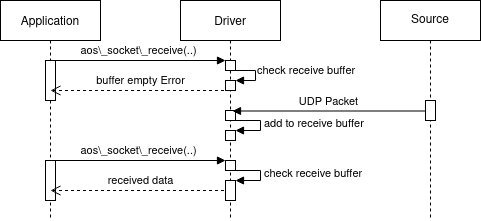
\includegraphics{networking/img/Sequence_Receive.png}
    }
    \caption{Receiving Data from a Remote Source}
    \label{fig:enet_recv}
\end{figure}

Similar to its UDP sockets, the library also provides an interface for sending ICMP echo requests and handling echo replies. For each target IP address, the driver keeps track of the last sent request's seqno as well as the highest acknowledged seqno. When an application tries to send the next echo request, the driver either retransmits a not yet acknowledged request, or if all requests have been acknowledged, sends a new request. Additionally, an application can request the highest seqno that has been acknowledged so far. The methods surrounding ICMP sockets are analog to the ones surrouning UDP sockets. For a simple example of them being used, see \C{usr/ping/main.c}.

\hindsight{
If the explanation of ICMP sockets seems rushed, then that is because their implementation was a bit rushed too. In hindsight, it would have been better to already consider requirements for ICMP messages when first writing the \C{udp\_service} library. Unfortunately, I first designed a library catered only towards sending and receiving UDP packets and only after it was working did I add ICMP ports and a \C{ping} application.
}

Perhaps the simplest method in this library is \C{aos\_arp\_table\_get}. It simply writes the device's current ARP table to a target buffer. Due to its simplicity, the function does not require any kind of socket to be initialized. Instead, it creates a new channel to the ethernet driver, requests the current ARP table, copies it to the target address and frees all data it allocated:
\begin{mdframed}[style=myframe]
\begin{minted}[xleftmargin=\parindent,linenos,breaklines]{C}
char *msg = malloc(2048);
aos_arp_table_get(msg);
print(msg);
\end{minted}
\end{mdframed}

\comment{
While trying to verify my correct implementation of the various protocols and algorithms, I encountered several peculiar interactions with my laptop. For instance, any UDP checksum I computed was flagged as faulty by Wireshark and ultimately never made it to its destination. However, Wireshark also flagged any outgoint UDP traffic from my laptop as faulty too. What solved this issue was to simply set the checksum to 0.

Another, more confusing issue I encountered was that any application (\emph{netcat, python,\dots}) running on my laptop was unable to receive UDP data from the Toradex board, unless Wireshark was running. I was unable to find the cause of this issue, but I found it interesting nonetheless.
}


\subsection{Networking Utilities}
Using the \C{udp\_service} library described above, I implemented a small selection of networking related programs. All of them can be started from \C{josh}.

\subsubsection{The arp Application}
The \C{arp} application (\emph{or \emph{"arplication"} for short}) simply requests the current ARP table from the driver, prints it and then terminates. It takes no arguments, but it does its best to provide aesthetically pleasing output. Listing \ref{enet:pingdemo} illustrates a possible output of this application.

\subsubsection{The ping Application}
The application \C{ping} creates an ICMP socket and uses it to send ICMP echo requests to a target IP address. It continuously updates the user on any received acknowledgements and keeps transmitting until the requested number of packets have been acknowledged. Its first argument is the target IP addres, and its second argument is the number of packets to have acknowledged. While it does not provide advanced features like packet multicasting, packet scheduling or time measurements, it still has its use cases. For instance, it can be used to indirectly trigger ARP requests when used on a new destination. Listing \ref{enet:pingdemo} shows how an initially empty ARP table can be extended after pinging a new destination.

\begin{code}
\begin{mdframed}[style=shell]
\josh{arp}\\
=========== ARP Table ===========\\
=================================\\
\\
\josh{ping 169.254.6.85 3}\\
pinging 169.254.6.85, 3 times\\
packet 1 was acked\\
packet 2 was acked\\
packet 3 was acked\\
\\
\josh{arp}\\
=========== ARP Table ===========\\
169.254.6.85\ \ \ \ \ \ 3e:1f:f:7:3:1\\
=================================
\end{mdframed}
\caption{Demonstration of \C{ping} causing ARP lookups}
\end{code}
\label{enet:pingdemo}

\subsubsection{The echoserver}
Finally, for an application built on UDP sockets, we have the \C{echoserver}. It takes a single argument, namely the port on which the server is to listen for incoming data. It then keeps receiving data on that port, and responds to any incoming data by sending an exact duplication back to its origin. Any device connected to the board can then send UDP packets to it and receive the exact same payload as reply. Listing \ref{enet:echodemo} show a remote device connecting to and using the echoserver with netcat.

\begin{code}
\begin{mdframed}[style=shell]
\bash{nc -u 10.0.2.1 4999}\\
Grow up Mr. Bond\\
Grow up Mr. Bond\\
Shaken, not stirred\\
Shaken, not stirred
\end{mdframed}
\caption{Demonstration of the Echo Server}
\end{code}
\label{enet:echodemo}

An earlier version of the echoserver was built directly inside the ethernet driver. With it, the driver had a separate handler it used for UDP packets arriving on port 2521. This handler created a reply with identical payload and sent it back to the source. While this version is not present in the driver's current form, it can be added back by adding the line \C{#define STATIC\_UDP\_ECHO 1} to the file \C{usr/drivers/enet/enet\_handler.c}.

Due to its simplicity, the echo server will be the main component of all performance measurements carried out below.

\subsection{The M-Shell}
The last application built using my \C{udp\_service} library is \C{msh} -- the M-shell. It allows users to connect to josh, our operating system's shell, over the internet. Since josh got their name from James Bond, and my remote shell essentially serves as a way to issue orders to josh, it seemed fitting to name my shell after "M" -- James Bond's boss. Luckily, \C{msh} has much more direct control over josh than M over Bond, so users will not have to worry about josh violating international law or going rogue on a quest for revenge.

Starting \C{msh} is very similar to starting an echo server: it only takes the port to listen on as argument. Once started, it first spawns a new \C{josh} process. But unlike the regular \C{josh} process spawned automatically at startup, this one does not read from and write to the serial port. Instead, \C{msh} has two data channels with this new process, one for \C{stdin} and one for \C{stdout}. Now \C{msh} can send any input for \C{josh} through one data channel and receive the output from the other one.

After spawning its own \C{josh} instance, \C{msh} then listens for incoming data on the specified port. It responds to the first message with a welcome message, but afterwards it simply forwards any UDP data to \C{josh} and sends any output it receives from \C{josh} back to the remote user.

Figure \ref{fig:msh_design} shows how this design works when a user attempts to evaluate the command \C{"echo a"} over my remote shell. It also illustrates an unexpected peculiarity: \C{josh} immediately writes every input it receives back to its \C{stdout} in order to give the user an immediate response to what they are typing. My remote shell will therefore also immediately echo every command it receives, and only then will it send back the output the command. To avoid confusion, the user is advised to disable their own terminal emulator from echoing back any key stroke. For a more responsive shell it is also advised to configure the terminal emulator to send each character immediately instead of sending data by lines. See listing \ref{enet:msh_demo} for an example of a user setting these recommended options and connecting to and using \C{msh}.

\begin{figure}[H]
\centering
    %\scalebox{0.9} {
    \resizebox{\textwidth}{!} {
        \includesvg{networking/img/msh_design.svg}
        %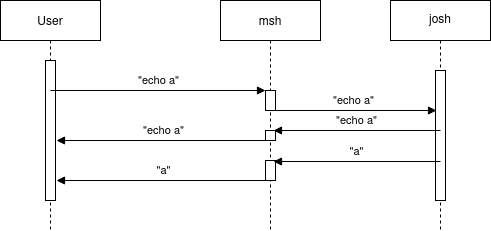
\includegraphics{networking/img/msh_design.png}
    }
    \caption{Receiving Data from a Remote Source}
    \label{fig:msh_design}
    
\end{figure}

\begin{code}
\begin{mdframed}[style=shell]
\bash{stty -icanon -echo \&\& nc -u 10.0.2.1 5000}\\
\\
\ m\ \ \ \ m\ \ mmmm\ \ m\ \ \ \ m\\
\ \#\#\ \ \#\# \#"\ \ \ " \#\ \ \ \ \#\\
\ \# \#\# \# "\#mmm\ \ \#mmmm\#\\
\ \# "" \#\ \ \ \ \ "\# \#\ \ \ \ \#\\
\ \#\ \ \ \ \# "mmm\#" \#\ \ \ \ \#\\
\\
\josh{@2 arp}\\
=========== ARP Table ===========\\
169.254.6.85\ \ \ \ \ \ 3e:1f:f:7:3:1\\
=================================\\
\end{mdframed}
\caption{Setting Recommended Settings and Using netcat to Connect to \C{msh}}
\end{code}
\label{enet:msh_demo}

An especially cool thing about this remote shell is that with the above command, it really does provide the exact same experience as using \C{josh} directly on the board itself. Not only do the color escape codes work seamlessly, but also the arrow keys, backspace and CTRL+L to clear all work as well.

\subsection{Performance Measurements}
Since UMP messages offer the most flexibility among the implemented features, I carried out all of my performance measurements by having the Toradex board run one or many UMP echo servers. On a connected computer I then ran python scripts to send messages of various length to the board and measure how long it takes for the echo reply to be received.

\subsubsection{Single Server}
For the first benchmark I had one echoserver running on the Toradex board. On my laptop I then ran a python script which sent messages of increasing payload size. For every message it sent, it measured how long it took for the corresponding answer to arrive. Each message size was sent a total of $4'096$ times and the response time was averaged over all iterations. Lastly, for the messages themselves I used part of the lyrics to \emph{Fool for Love} by \emph{Lord Huron}. While that last detail is not directly relevant to the results themselves, it is a great song and I will use every chance to mention it. 

I ran this first experiment a total of three times. One time the echo server was running on core 0, once it was running on core 1 and once it was running inside the ethernet driver itself (\emph{see Figure \ref{fig:single_echo})}. Unsurprisingly, the server inside the driver had by far the lowest latency. Since the incoming data never had to make the detour to a separate process before being sent back, the board was able to respond the quickest out of all tested configurations. Furthermore, running the echo server outside the driver but on the same core results in the highest latency, while running it on a separate core is only slightly worse than running it inside the driver. These results are not surprising, as processes sharing the same core can often interfere with each other, leading to performance losses and thus higher latency.
%Additionally, our measurements from section \ref{mp:perf_subs} also showed better performance for UMP channels than for LMP, 

\begin{figure}[H]
\centering
    \resizebox{\textwidth}{!} {
        \includesvg{networking/img/single_echo.svg}
    }
    \caption{Benchmarking Latency for a Single Echo Server Instance}
    \label{fig:single_echo}
\end{figure}

\subsubsection{Multiple Servers}
To benchmark my network stack's latency under a higher load, I had multiple echo servers running on different ports. Based on my previous results I ran all of them on cores 1-3. For each running server I had one agent on my laptop repeating the previous test. This experiment was done with up to 10 echo servers, each communicating with a separate measuring agent. Figure \ref{fig:para_echo} shows the average latency for varying numbers of servers and different message sizes.

\begin{figure}[H]
\centering
    \resizebox{\textwidth}{!} {
        \includesvg{networking/img/para_echo.svg}
    }
    \caption{Latency for Multiple Single Echo Server Instances}
    \label{fig:para_echo}
\end{figure}

Unsurprisingly, the latency increases significantly with more servers running in parallel. Especially for short messages, a low number of threads produces much better performance, as even very short waiting periods for any of the servers have an immediately visible effect on the overall latency. For larger message sizes on the other hand, even messages that get handled without ever waiting for the driver take quite a while to travel to the echo server, back to the driver and then back to the remote device. As a result, a higher number of running servers is much less noticeable. In fact, for very long messages, the latency was virtually identical for all measurements taken with 1-3 running servers.

\subsubsection{Bandwidth Measurements}
While low latency certainly is desirable, it is useless without an acceptable bandwidth to go along with. My last measurements were therefore trying to find my network stack's maximum bandwidth. For this I had one thread on my laptop send packets of size 128 to the Toradex board at a constant bandwidth for 5 minutes, while another thread was receiving and counting all the data coming in response. Meanwhile, there was a single echo server running on the Toradex board's core 1. This was then repeated for several different bandwidths, producing the red results shown in Figure \ref{fig:bw_echo}.

\begin{figure}[H]
\centering
    \resizebox{\textwidth}{!} {
        \includesvg{networking/img/bw_udp.svg}
    }
    \caption{Bandwidth of a Single Echo Server Instance}
    \label{fig:bw_echo}
\end{figure}

As can be seen, my network stack can easily achieve bandwidths of up to $190 \frac{MB}{s}$, as it was comfortably able to keep up with the load up to that point. For loads beyond that, the initial version of my stack was no longer able to keep up, and for roughly $1.2 \frac{GB}{s}$ it stopped working entirely, because the nameservice shut it down. Since my ethernet driver's initial version always checked for new packets before it checked for incoming RPCs, a too high network load lead to the ethernet driver being unable to respond to any other processes on the device itself. In response, the nameserver assumed the driver had stopped working and removed it. Luckily, this issue was easy to ammend simply by reprogramming the ethernet driver to first dispatch any RPCs before checking for incoming packets.

Indeed, implementing this small change inside the ethernet driver produces the much better blue results. The driver is now able to reach almost twice as high bandwidths, and even when the echo server is no longer able to keep up with the offered load, the driver does not stop working entirely. Instead it still achieves bandwidths higher than the previous driver version did most of the time.

% stty -icanon -echo && nc -u 10.0.2.1 1525